\documentclass[a4paper]{article}
\usepackage{cmap}					% поиск в PDF
\usepackage[T2A]{fontenc}			% кодировка
\usepackage[utf8]{inputenc}			% кодировка исходного текста
\usepackage[english,russian]{babel}	% локализация и переносы

\usepackage{tikz}

\usepackage{bm}
\usepackage{amsmath,amsfonts,amssymb,amsthm,mathtools} % AMS
\usepackage{icomma}

\usepackage{xcolor}
\usepackage{array}
\usepackage{svg}

\usepackage{hyperref}
\usepackage{longtable}
\usepackage{listings}

\usepackage{pdfpages}

\usepackage[left=3cm,right=1cm,top=2cm,bottom=2cm,bindingoffset=0cm]{geometry}
\linespread{1.3}

\newcolumntype{C}[1]{>{\centering\arraybackslash}p{#1}}
	
\definecolor{dkgreen}{rgb}{0,0.6,0}
\definecolor{gray}{rgb}{0.5,0.5,0.5}
\definecolor{mauve}{rgb}{0.58,0,0.82}

\lstset{
	language=SQL,
	aboveskip=3mm,
	belowskip=3mm,
	showstringspaces=false,
	columns=flexible,
	basicstyle={\small\ttfamily},
	numbers=none,
	numberstyle=\tiny\color{gray},
	keywordstyle=\color{blue},
	commentstyle=\color{dkgreen},
	stringstyle=\color{mauve},
	breaklines=true,
	breakatwhitespace=true,
	tabsize=2,
	captionpos=t,
	keepspaces
}



\begin{document}
	

\includepdf{title.pdf}
	
\tableofcontents
\setcounter{page}{1}
\newpage
	
\section{Формулировка задания}
Целью данной работы является проектирование базы данных для индексирования геоданных: оптических и радарных космических снимков, а так же соответствующих им векторных масок; с целью дальнейшего их использования в создании алгоритмов машинного обучения и новых масок.
При создании базы данных необходимо учитывать типовые операции, проводящиеся со снимками в рамках процесса разработки алгоритмов, а так же обеспечить расширяемость на новые типы снимков.

\section{Описание предметной области}
Многие практические задачи обработки ДЗЗ, такие как сегментация подстилающей поверхности, устранение дефектов снимков, улучшение разрешения и т.д., не могут быть решены классическими алгоритмами обработки. Поэтому, всё чаще используются алгоритмы на основе машинного обучения, причём, как правило, типа ``supervised learning''.
Данные алгоритмы требуют больших объёмов тренировочных (размеченных) данных, например для сегментации поверхности --- это созданные вручную маски поверхности.
Для того, чтобы оптимизировать время разработки новых моделей, требуется наладить конвейер обработки данных и моделей.
В рамках этой работы рассмотрено проектирование базы данных для такого конвейера.

\subsection{Некоторые определения}
\begin{itemize}
	\item Продукт --- совокупность одного или нескольких снимков, обладающих некоторыми общими свойствами.
		Например: стереопары --- это пары снимков одной территории, снятые примерно в одно время с разных ракурсов (углов).
		Позволяют строить стереомодели объектов.
	\item Выборка --- совокупность продуктов, и, иногда, векторных масок к ним, отобранная для обучения или тестирования алгоритма.
	\item Сенсор --- в узком смысле --- спутник, производящий съемку.
		В широком смысле --- система спутников одного вида, обладающих одинаковыми свойствами (например --- пространственным разрешением).
	\item Векторная маска / разметка / вектор --- полигон или множество полигонов, имеющих географическую привязку, и описывающих какие-то объекты / типы территории на снимках.
\end{itemize}

\subsection{Типовые операции с данными}
\subsubsection{Тематический отдел}
Тематический отдел занимается созданием разметки.
Типовые операции тематического отдела:
\begin{itemize}
	\item Получение продукта по географическим координатам от определённого сенсора за определённый временной промежуток.
	\item Получение продукта по исходному идентификатору.
	\item Добавление новой векторной маски.
	\item Получение стабильной версии модели машинного обучения для произведения полуавтоматической разметки.
	\item Добавление свойств продукта.
	\item Формирование выборки.
\end{itemize}

\subsubsection{Алгоритмический отдел}
Алгоритмический отдел занимается созданием алгоритмов для обработки.
Типовые операции алгоритмического отдела:
\begin{itemize}
	\item Формирование выборки (иногда).
	\item Получение, первичная обработка выборки.
	\item Добавление новых моделей машинного обучения.
	\item Добавление новых версий моделей машинного обучения.
	\item Отслеживание версий экспериментов (интеграция с VCS, например с GIT).
\end{itemize}

\section{Модели базы данных}
\subsection{Концептуальная модель БД}
На основе приведённых выше типовых операций, а так же общей структуры предметной области, была составлена концептуальная модель БД.
Для того, чтобы не засорять схему, атрибуты не были указаны на ней, а вместо этого представлены в разделе \nameref{attributes_definitions}

\begin{figure}[h]
	\centering
	\includesvg[width=\columnwidth]{./images/ER.svg}
	\caption{Концептуальная модель БД}
\end{figure}

\subsection{Список сущностей}
В ходе моделирования, были выделены следующие сущности:
\begin{itemize}
	\item Продукт
	\item Снимок
	\item Источник
	\item Снимок НЦОМЗ
	\item Снимок ``Planet''
	\item Снимок ``DG''
	\item Вектор
	\item Автор
	\item Обработчик
	\item Выборка
	\item Модель
	\item Эксперимент
	\item Класс вектора
\end{itemize}

\subsection{Описание атрибутов}
\label{attributes_definitions}
В следующих таблицах приводится более подробное описание атрибутов каждой сущности.


\begin{longtable}{|C{0.20\textwidth}|p{0.75\textwidth}|}
	\caption{Таблица атрибутов} \\
	
	\hline
	Атрибут & \centering\arraybackslash Описание \\
	\hline
	\endfirsthead
	\hline
	\endhead
	\hline
	\endfoot
	
	\multicolumn{2}{|c|}{Описание атрибутов продукта} \\
	\hline
	type & Тип продукта. На данный момент всего два типа: стерео и обычный, но может значительно пополняться в будущем \\
	\hline
	images & Множество снимков, входящих в данный продукт \\
	\hline
	delivery\_id & Номер поставки, нужен для отслеживания в случае обнаружения некорректных поставок \\
	\hline
	indexed\_datetime & Время добавления в БД \\
	\hline

	\multicolumn{2}{|c|}{Описание атрибутов источника снимка} \\
	\hline
	name & Название данного источника \\
	\hline
	additional\_fields & Список полей (атрибутов), не входящих в сущность ``Снимок'', но присутствующих в отдельной таблице снимков для этого источника. Например, cloud\_map для ``Planet'' \\
	\hline

	\multicolumn{2}{|c|}{Описание атрибутов снимка} \\
	\hline
	id & Внутренний идентификатор снимка (так же первичный ключ) \\
	\hline
	external\_id &  Внешний идентификатор снимка (используется для индексации снимков в системе, откуда он был получен) \\
	\hline
	source & Источник, из которого был получен снимок \\
	\hline
	sat & Спутника с которого был получен снимок \\
	\hline
	capture\_conditions & Дополнительные параметры съёмки: угол наклонения орбиты, солнца и т.д. \\
	\hline
	captured\_datetime & Дата и время, в которое был сделан снимок (усреднённое значение) \\
	\hline
	processed\_datetime & Дата и время, когда снимок был обработан во внешней системе обработки \\
	\hline
	type & Тип снимка: мультиспектральный, панхроматический, или результат паншарпенинга \\
	\hline
	geometry & Геометрия снимка на поверхности земли (геопривязка) \\
	\hline
	path & Путь к самому снимку \\
	\hline
	ql\_path & Путь к снимку сжатому в несколько раз, для быстрого ``поверхностного'' просмотра \\
	\hline
	other\_paths & Пути к другим файлам, которые шли в поставке вместо со снимком \\
	\hline

	\multicolumn{2}{|c|}{Описание атрибутов снимка ``Planet''} \\
	\hline
	cloud\_map & Полигон, описывающий облака и тени от облаков, присутствующие на снимке \\
	\hline
	
	\multicolumn{2}{|c|}{Описание атрибутов снимка ``DG''} \\
	\hline
	cloud\_map & Полигон, описывающий облака и тени от облаков, присутствующие на снимке \\
	\hline
	stereo\_number & Номер стереоснимка (если тип продукта стерео), иначе -1 \\
	\hline

	\multicolumn{2}{|c|}{Описание атрибутов снимка НЦОМЗ} \\
	\hline
	hash & Уникальный хэш первичной обработки снимка \\
	\hline
	scene & Номер сцены в пролёте \\
	\hline
	selected & Является ли данный снимок ``отобранным'' --- т.е. приемлемым для работы \\
	\hline
	defects & Список дефектов данного снимка \\
	\hline

	\multicolumn{2}{|c|}{Описание атрибутов вектора} \\
	\hline
	datetime & Дата и время создания данного вектора \\
	\hline
	authors & Множество сущностей (людей и других алгоритмов), принимавших участие в создании вектора \\
	\hline
	class & Класс, который выделен данным вектором \\
	\hline
	image & Изображение, на которое был создан данный вектор \\
	\hline
	other & Дополнительные поля \\
	\hline
	geometry & Непосредственно полигоны, задающие данный вектор \\
	\hline

	\multicolumn{2}{|c|}{Описание атрибутов класса вектора} \\
	\hline
	short\_description & Краткое описание данного класса вектора. Например: лес, озеро, дефект матрицы и т.д. \\
	\hline
	description & Полное описание данного класса. Например: ``Дефект матрицы 2-го типа, обычно вызванный внутренними перебоями питания КА'' \\
	\hline
	color & Цвет, которым нужно выделять данный класс на ситуационной карте \\
	\hline

	\multicolumn{2}{|c|}{Описание атрибутов выборки} \\
	\hline
	name & ФИО автора \\
	\hline
	contacts & Каналы для связи \\
	\hline
	%\caption{Описание атрибутов автора}
	\hline
	images & Список снимков в данной выборке \\
	\hline
	masks & Список векторных масок в данной выборке \\
	\hline
	parent & Родительская выборка. Выборки образуют структуру похожую на лес, т.е. множество деревьев \\
	\hline

	\multicolumn{2}{|c|}{Описание атрибутов эксперимента} \\
	\hline
	author & Автора эксперимента \\
	\hline
	datetime & Время начала эксперимента \\
	\hline
	git\_commit & Хэш коммита в VCS, отвечающий данному эксперименту \\
	\hline
	dataset & Выборка, использовавшаяся в данном эксперименте \\
	\hline
	parent & Родительский эксперимент (эксперименты образуют структуру типа леса, т.е. множества деревьев) \\
	\hline
	models & Список моделей, порождённых данным экспериментом \\
	\hline

	\multicolumn{2}{|c|}{Описание атрибутов модели} \\
	\hline
	type & Тип модели: сегментация, детекция, регрессия и т.д. \\
	\hline
	paths & Список путей к файлам модели (обученная модель представляет из себя бинарный файл, но может быть сохранена в разных форматах, иногда без возможности конвертации между ними) \\
	\hline
	other & Дополнительные атрибуты \\
	\hline
\end{longtable}




\subsection{Логическая модель БД}
Следующим шагом было построение логической модели БД, подробнее отражающей реализацию концепции в рамках реляционной модели.
Связи типа ``многие-ко-многим'' реализованы с помощью отдельных связующих таблиц.
Связи типа ``один-к-одному'' реализованы с помощью техники выносного первичного ключа.
Древовидные структуры (эксперименты и выборки) реализованы с помощью хранения ссылки на родительский элемент.

\begin{figure}[h]
	\centering
	\includesvg[width=\columnwidth]{./images/Logic.svg}
	\caption{Логическая модель БД}
\end{figure}


\subsection{Физическая модель БД}
В качестве СУБД для реализации была выбрана PostgreSQL.
Основным фактором при выборе СУБД было наличие средств / библиотек для работы с геометрическими типами данных.
В PostgreSQL такой инструмент есть и является очень хорошо развитым.
PostGIS позволяет эффективно осуществлять геометрические запросы, например по пересечению, объединению, вхождению и т.д.
Кроме того, в PostGIS в виде хранимых процедур реализованы и другие функции для работы с геометрией: перепроецирование, нахождение площади произвольных полигонов и т.д.

\begin{figure}[h]
	\centering
	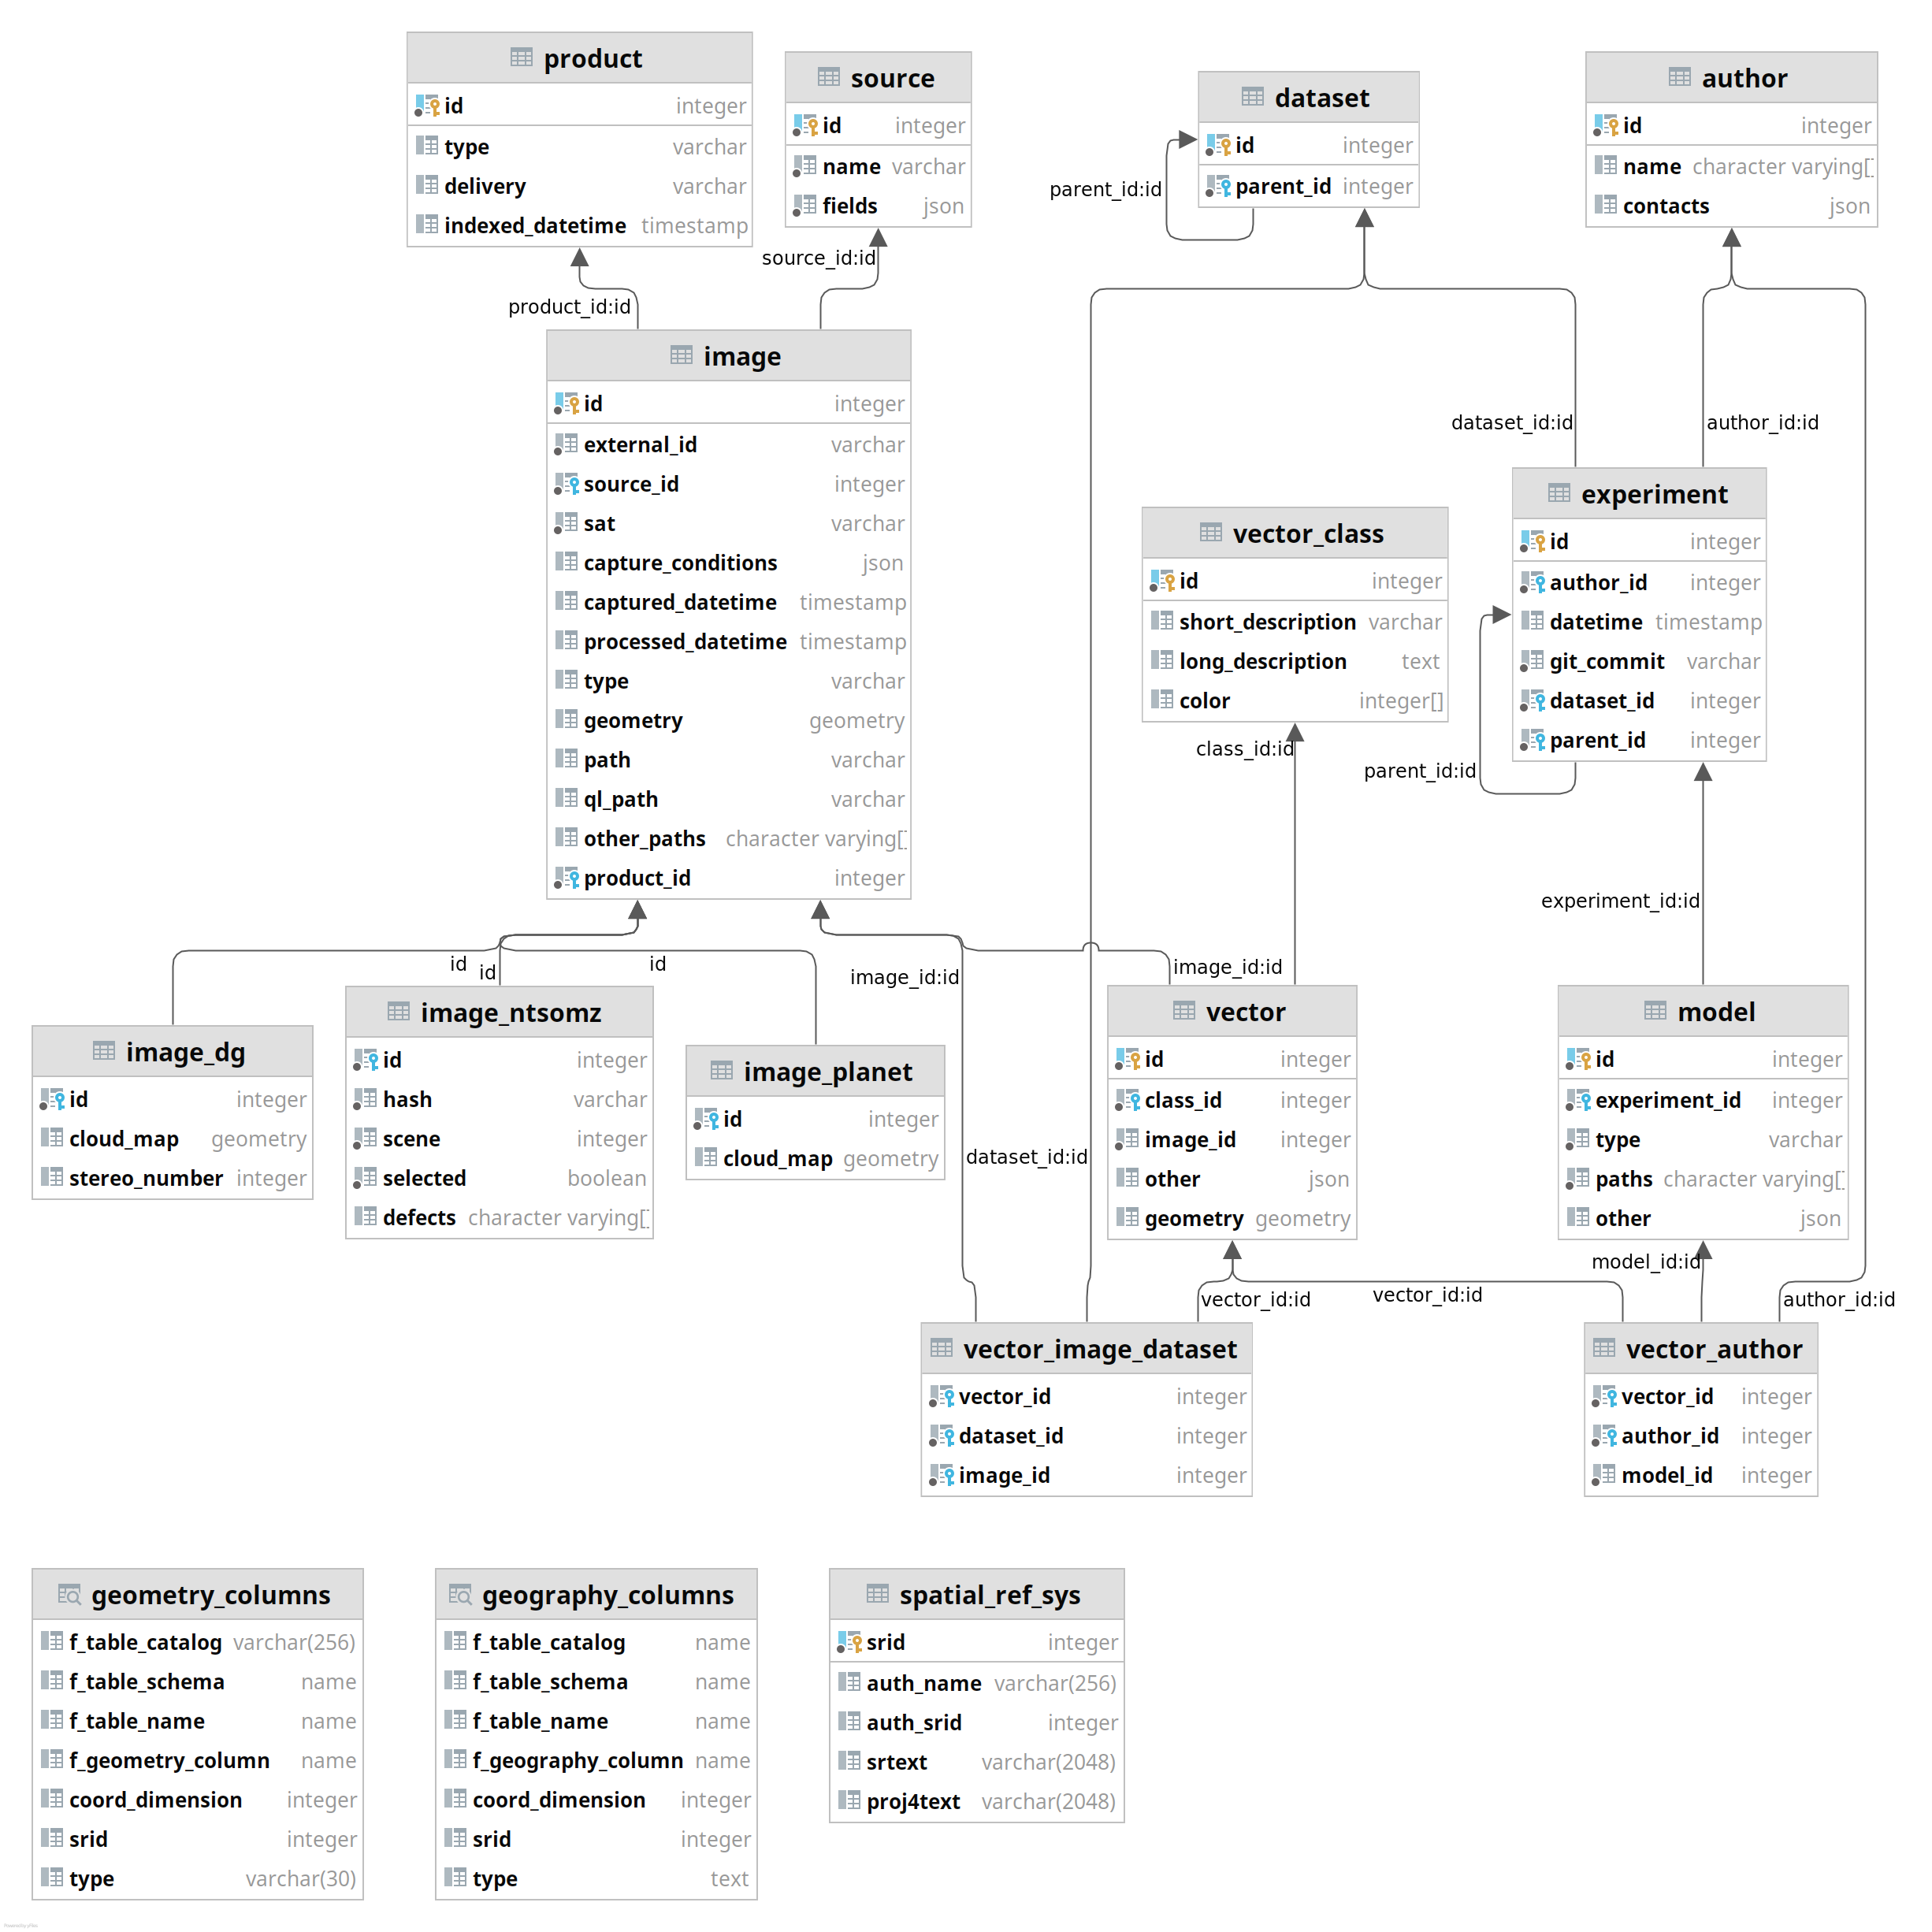
\includegraphics[width=\columnwidth]{./images/Physics.png}
	\caption{Физическая модель БД в СУБД PostgreSQL}
\end{figure}


\section{Реализация базы данных}
В данном разделе представлена реализация структуры базы данных, а так же некоторых типовых операций.

\subsection{Реализация структуры БД}
\lstinputlisting[caption={Создание структуры БД}]{../database.sql}

\subsection{Заполнение БД}
\lstinputlisting[caption={Заполнение БД}, label={lst:insertion}]{../insertion.sql}
Листинг \ref{lst:insertion} содержит минимальный пример заполнения БД.
Здесь создаётся 3 типа источника в соответствии с таблицами источников, добавляется 3 продукта, содержащих по одному снимку.
Затем добавляется один класс вектора, и 4 вектора, принадлежащих данному классу.
Из всех векторов и снимков затем создаётся один датасет, и три эксперимента, его использующих, причём два первых эксперимента образуют одну ветку, а третий вторую.
Каждый из экспериментов порождает по одной модели.

\subsection{Реализация типовых операций}
В данном разделе представлены примеры некоторых операций, которые можно производить в рамках созданной базы данных.

\begin{lstlisting}[captionpos=b, caption={Получение изображения, пересекающегося с заданным полигоном, являющегося отобранным для работы и снятого в конкретный промежуток времени.}]
select image.id, image.path from image
inner join image_ntsomz on image.id = image_ntsomz.id
where
	st_intersects(st_geomfromewkt('POLYGON ((35 10, 45 45, 15 40, 10 20, 35 10), (20 30, 35 35, 30 20, 20 30))'), image.geometry) and
	selected=true and
	make_date(2019, 7, 03) <= date(captured_datetime) and
	date(captured_datetime) <= make_date(2019, 7, 10);
\end{lstlisting}

\begin{lstlisting}[captionpos=b, caption={Получение стереопары по данному id изображения}]
select image.id from image
where image.product_id in (select image1.product_id from image as image1 where image1.id = 1);
\end{lstlisting}

\begin{lstlisting}[captionpos=b, caption={Получение всех моделей, порождённых данной веткой экспериментов}]
with recursive ctename as (
	select experiment.parent_id as expirement_parent_id, model.id as model_id from experiment
	inner join model on experiment.id = model.experiment_id
	where experiment.id = 2
	UNION
		select experiment.id, model.id from experiment
		inner join ctename on ctename.expirement_parent_id = experiment.id
		inner join model on experiment.id = model.experiment_id
)
select model_id from ctename;
\end{lstlisting}

\begin{lstlisting}[captionpos=b, caption={Получение всех пар изображений для данного датасета}]
select image_id, vector_id from vector_image_dataset
where dataset_id = 1
group by image_id, vector_id;
\end{lstlisting}

\section{Заключение}
В данной работе было рассмотрено проектирование БД для обеспечения работы конвейера обработки данных при обучении алгоритмов машинного обучения в контексте работы с геоданными.
Хотя БД и является центральной частью этого конвейера, для его полноценной работы требуется ещё множество иных программных решений: начиная от интерфейсов для работы тематического отдела (плагины встраиваемые в ПО типа QGis и ArcGis) и заканчивая полноценным фреймворком для ЯП Python для нужд алгоритмического отдела.
Разработка данных средств, конечно же, выходит за рамки этой работы и этого семестра, однако, возможно, будет осуществлена в будущем.
	
\end{document}